\subsection{与正合列相伴的类的性质}

命题 3. --- 设

\begin{enumerate}
\def\labelenumi{(\arabic{enumi})}
\setcounter{enumi}{5}
\tightlist
\item
\end{enumerate}

\[
0 \rightarrow \mathrm{P} \rightarrow \mathrm{S} _ {m} \rightarrow \mathrm{S} _ {m - 1} \rightarrow \dots \rightarrow \mathrm{S} _ {1} \stackrel {\lambda_ {n}} {\rightarrow} \mathrm{N} \rightarrow 0\tag{7}
\]

\[
0 \rightarrow \mathrm{N} \xrightarrow {\mu} \mathrm{R} _ {n} \rightarrow \mathrm{R} _ {n - 1} \rightarrow \dots \rightarrow \mathrm{R} _ {1} \rightarrow \mathrm{M} \rightarrow 0
\]

为两个左 A-模正合列，其类分别为 \(\theta\in\mathrm{Ext}_{\mathbf{A}}^{m}(\mathbf{N},\mathbf{P})\) 与 \(\theta^{\prime}\in\mathrm{Ext}_{\mathbf{A}}^{n}(\mathbf{M},\mathbf{N})\) 。 \(\mathrm{Ext}_{\mathbf{A}}^{m+n}(\mathbf{M},\mathbf{P})\) 中与正合列

\[
0 \to \mathrm{P} \to \mathrm{S} _ {m} \to \dots \to \mathrm{S} _ {1} \xrightarrow {\mu \circ \lambda} \mathrm{R} _ {n} \to \dots \to \mathrm{R} _ {1} \to \mathrm{M} \to 0\tag{8}
\]

相伴的类是复合积 \(\theta\circ\theta'\) 。

选取交换图

\[
\begin{array}{c} 0 \longrightarrow \mathrm{P} \longrightarrow \mathrm{I} ^ {0} (\mathrm{P}) \longrightarrow \dots \longrightarrow \mathrm{I} ^ {m - 1} (\mathrm{P}) \xrightarrow {\delta_ {\mathrm{P}} ^ {m - 1}} \mathrm{I} ^ {m} (\mathrm{P}) \\ 0 \longrightarrow \mathrm{P} \longrightarrow \mathrm{S} _ {m} \longrightarrow \dots \longrightarrow \mathrm{S} _ {1} \xrightarrow {\lambda} \mathrm{N} \longrightarrow 0, \end{array}
\]

\[
\begin{array}{c c c c c c c c c c c c} 0 \longrightarrow & \mathrm{N} & \stackrel {{e _ {\mathrm{N}}}} {{\longrightarrow}} & \mathrm{I} ^ {0} (\mathrm{N}) & \longrightarrow & \dots & \longrightarrow & \mathrm{I} ^ {n - 1} (\mathrm{N}) & \longrightarrow & \mathrm{I} ^ {n} (\mathrm{N}) \\ & \uparrow_ {1 _ {\mathrm{N}}} & & v ^ {0} \uparrow & & & & v ^ {n - 1} \uparrow & & v ^ {n} \uparrow \\ 0 \longrightarrow & \mathrm{N} & \stackrel {{\mu}} {{\longrightarrow}} & \mathrm{R} _ {n} & \longrightarrow & \dots & \longrightarrow & \mathrm{R} _ {1} & \longrightarrow & \mathrm{M} & \longrightarrow & 0. \end{array}
\]

由于 \(\mathrm{I}^{m}(\mathrm{P})\) 是内射的，存在同态 \(h^{0}: \mathrm{I}^{0}(\mathrm{N}) \to \mathrm{I}^{m}(\mathrm{P})\) 使得 \(w^{m} = h^{0} \circ e_{N}\) ；由 X 第 49 页命题 3 bis， \(h^{0}\) 可延拓为复形的态射 \(h: \mathrm{I}(\mathrm{N}) \to \mathrm{I}(\mathrm{P})(-m)\) 。于是 \(w^{m} = h^{0} \circ e_{N} = h^{0} \circ v^{0} \circ \mu\) ，因此

\[
\delta_ {1} ^ {m - 1} \circ w ^ {m - 1} = w ^ {m} \circ \lambda = h ^ {0} \circ v ^ {0} \circ (\mu \circ \lambda),
\]

且下图是交换的：

\[
\begin{array}{l}0 \longrightarrow \mathrm{P} \longrightarrow \mathrm{I} ^ {0} (\mathrm{P}) \longrightarrow \dots \longrightarrow \mathrm{I} ^ {m - 1} (\mathrm{P}) \longrightarrow \mathrm{I} ^ {m} (\mathrm{P}) \longrightarrow \mathrm{I} ^ {m + 1} (\mathrm{P}) \longrightarrow \dots \longrightarrow \mathrm{I} ^ {m + n} (\mathrm{P})\\0 \longrightarrow \mathrm{P} \longrightarrow \mathrm{S} _ {m} \longrightarrow \dots \longrightarrow \mathrm{S} _ {1} \underset {\mu \circ \lambda} {\longrightarrow} \mathrm{R} _ {n} \longrightarrow \mathrm{R} _ {n - 1} \longrightarrow \dots \longrightarrow \mathrm{M} \rightarrow 0\end{array}
\]

其中 \(t^0 = h^0 \circ v^0\) , \(t^1 = (-1)^m h^1 \circ v^1, \ldots, t^i = (-1)^{mi} h^i \circ v^i, \ldots, t^n = (-1)^{mn} h^n \circ v^n\) 。与 (6) 相伴的类 \(\theta\) 是 \((-1)^{m(m+1)/2} w^m \in \text{Homgr}_A^m(\mathbf{N}, \mathbf{l}(\mathbf{P}))\) 的类，因此经同构 \(a_{\mathbf{N},\mathbf{P}}\) 对应于 \((-1)^{m(m+1)/2} h \in \text{Homgr}_A^m(\mathbf{l}(\mathbf{N}), \mathbf{l}(\mathbf{P}))\) 的类；与 (7) 相伴的类 \(\theta'\) 是 \((-1)^{n(n+1)/2} v^n \in \text{Homgr}_A^m(\mathbf{M}, \mathbf{l}(\mathbf{N}))\) 的类，与 (8) 相伴的类是 \((-1)^{(m+n)(m+n+1)/2} t^n \in \text{Homgr}_{m+n}^m(\mathbf{M}, \mathbf{l}(\mathbf{P}))\) 的类，于是由复合积的定义（X，第 114 页）及公式得出结论

\[
m (m + 1) / 2 + n (n + 1) / 2 = (m + n) (m + n + 1) / 2 - m n.
\]

\begin{enumerate}
\def\labelenumi{\arabic{enumi}.}
\setcounter{enumi}{3}
\tightlist
\item
  --- 考虑一个 A-模的交换图，它具有正合
\end{enumerate}

行

\pandocbounded{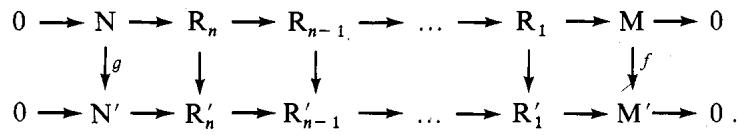
\includegraphics[keepaspectratio]{images/part001_b790ce53.jpg}}

设 θ（相应地，θ′）为第一行（相应地，第二行）在下式中的类

\[
\operatorname{Ext} _ {\mathbf {A}} ^ {n} (\mathbf {M}, \mathbf {N}) \quad \left(\text { resp.   } \operatorname{Ext} _ {\mathbf {A}} ^ {n} (\mathbf {M} ^ {\prime}, \mathbf {N} ^ {\prime})\right).
\]

在 \(\operatorname{Ext}_{\mathbf{A}}^{n}(\mathbf{M}, \mathbf{N}')\) 中，有 \(\theta' \circ f = g \circ \theta\) 。

事实上，考虑一个交换图

\pandocbounded{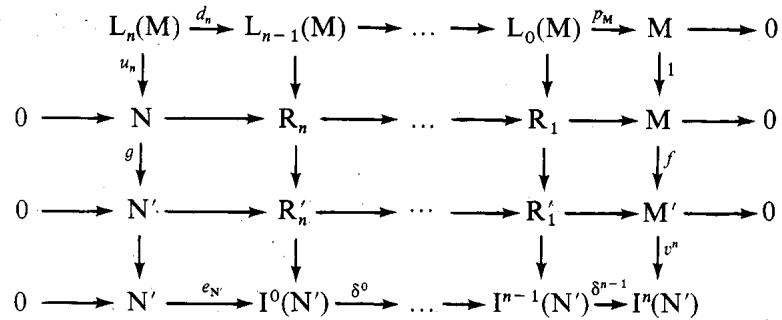
\includegraphics[keepaspectratio]{images/part001_126cf8d3.jpg}}

根据定义， \(\theta' \circ f\) 是 \((-1)^{n(n+1)/2} v^n \circ f \circ p_M \in \text{Homgr}^n (\text{L(M)}, \text{I(N')})\) 的类，而 \(g \circ \theta\) 是 \((-1)^{n(n+1)/2} e_{N'} \circ g \circ u_n\) 的类。将引理 1 应用于该图两端的行，这两个类相等。

推论 1. --- 考虑一个具有正合行的交换图

\[
\begin{array}{c c c c c c c c} 0 \longrightarrow & \mathrm{N} \longrightarrow & \mathrm{R} _ {n} \longrightarrow & \dots & \longrightarrow & \mathrm{R} _ {1} \longrightarrow & \mathrm{M} \longrightarrow & 0 \\ & ^ {1} \downarrow & & & \downarrow & & ^ {1} \downarrow \\ 0 \longrightarrow & \mathrm{N} \longrightarrow & \mathrm{R} _ {n} ^ {\prime} \longrightarrow & \dots & \longrightarrow & \mathrm{R} _ {1} ^ {\prime} \longrightarrow & \mathrm{M} \longrightarrow & 0; \end{array}
\]

图的两行在 \(\operatorname{Ext}_{\mathbf{A}}^{n}(\mathbf{M},\mathbf{N})\) 中有相同的相伴类。

推论 2. --- 设

\[
0 \rightarrow \mathrm{N} \xrightarrow {f _ {n - 1}} \mathrm{R} _ {n} \xrightarrow {f _ {n}} \mathrm{R} _ {n - 1} \rightarrow \dots \xrightarrow {f _ {2}} \mathrm{R} _ {1} \xrightarrow {f _ {1}} \mathrm{M} \rightarrow 0
\]

是一个正合列， \(\theta\in\mathrm{Ext}_{\mathbf{A}}^{n}(\mathbf{M},\mathbf{N})\) 为其相伴的类， \(a_{1},\ldots,a_{n+1}\) 为 \(k\) 的可逆元。与正合列

\[
0 \rightarrow \mathrm{N} \xrightarrow {a _ {n + 1} f _ {n + 1}} \mathrm{R} _ {n} \xrightarrow {a _ {n} f _ {n}} \mathrm{R} _ {n - 1} \rightarrow \dots \xrightarrow {a _ {2} f _ {2}} \mathrm{R} _ {1} \xrightarrow {a _ {1} f _ {1}} \mathrm{M} \rightarrow 0
\]

相伴的类是 \((a_{1}^{-1}a_{2}^{-1}\dots a_{n + 1}^{-1})\theta .\)

事实上，我们有一个交换图

\[
\begin{array}{c} 0 \longrightarrow \mathrm{N} \xrightarrow {a _ {n + 1} f _ {n + 1}} \mathrm{R} _ {n} \longrightarrow \dots \longrightarrow \mathrm{R} _ {2} \xrightarrow {a _ {2} f _ {2}} \mathrm{R} _ {1} \xrightarrow {a _ {1} f _ {1}} \mathrm{M} \longrightarrow 0 \\ \Biggl \downarrow a _ {1} \dots a _ {n + 1} \quad \Biggl \downarrow a _ {1} \dots a _ {n} \quad \Biggl \downarrow a _ {1} a _ {2} \quad \Biggl \downarrow a _ {1} \quad \Biggl \downarrow 1 \\ 0 \longrightarrow \mathrm{N} \xrightarrow {f _ {n + 1}} \mathrm{R} _ {n} \longrightarrow \dots \longrightarrow \mathrm{R} _ {2} \xrightarrow {f _ {2}} \mathrm{R} _ {1} \xrightarrow {f _ {1}} \mathrm{M} \longrightarrow 0. \end{array}
\]

然后应用该命题。

推论 3. --- 设 \(0 \to \mathbf{N} \xrightarrow{f_{n+1}} \mathbf{R}_{n} \xrightarrow{f_{n}} \cdots \to \mathbf{R}_{1} \xrightarrow{f_{1}} \mathbf{M} \to 0\) 为一个正合列， \(\theta\) 为它在 \(\operatorname{Ext}_{\mathbf{A}}^{n}(\mathbf{M}, \mathbf{N})\) 中的类， \(u: \mathbf{M}' \to \mathbf{M}\) 与 \(v: \mathbf{N} \to \mathbf{N}'\) 为两个 A-模同态。

\begin{enumerate}
\def\labelenumi{\alph{enumi})}
\tightlist
\item
  元素 \(v \circ \theta\) （属于 \(\operatorname{Ext}_{\mathbf{A}}^{n}(\mathbf{M}, \mathbf{N}')\) ）等于正合列
\end{enumerate}

\[
0 \rightarrow \mathrm{N} ^ {\prime} \xrightarrow {f _ {n + 1} ^ {\prime}} \mathrm{R} _ {n} ^ {\prime} \xrightarrow {f _ {n} ^ {\prime}} \mathrm{R} _ {n - 1} \xrightarrow {f _ {n - 1}} \dots \rightarrow \mathrm{R} _ {1} \rightarrow \mathrm{M} \rightarrow 0,
\]

的类，其中 \(R_{n}^{\prime}\) 是 A-模 \(R_{n} \oplus N^{\prime}\) 除以由诸对 \((f_{n+1}(x), -v(x))\) （ \(x \in N\) ）所构成的子模而得的商模，而 \(f_{n+1}^{\prime}\) (相应地， \(f_{n}^{\prime}\) )由典范单射（相应地，由 \((f_{n}, 0)\) ）通过取商得到。

\begin{enumerate}
\def\labelenumi{\alph{enumi})}
\setcounter{enumi}{1}
\tightlist
\item
  元素 \(\theta \circ u\) （属于 \(\operatorname{Ext}_{\mathbf{A}}^{n}(\mathbf{M}^{\prime}, \mathbf{N})\) ）是正合列
\end{enumerate}

\[
0 \rightarrow \mathrm{N} \rightarrow \mathrm{R} _ {n} \rightarrow \dots \rightarrow \mathrm{R} _ {2} \xrightarrow {f _ {2} ^ {\prime \prime}} \mathrm{R} _ {1} ^ {\prime} \xrightarrow {f _ {1} ^ {\prime \prime}} \mathrm{M} ^ {\prime} \rightarrow 0,
\]

的类，其中 \(R_{1}^{\prime}\) 是纤维积 \(R_{1} \times_{M} M^{\prime}\) ，亦即（I，第 44 页） \(R_{1} \times M^{\prime}\) 中由对 \((x, y)\) （满足 \(f_{1}(x) = u(y)\) ）所构成的子模，而 \(f_{2}^{\prime\prime}\) (相应地， \(f_{1}^{\prime\prime}\) )由 \((f_{2}, 0)\) （相应地，由第二个投影）导出。

例如，我们来证明 \(a\) )。设 \(z\) 为 \(\mathbf{R}_{n}^{\prime}\) 中满足 \(f_{n}^{\prime}(z)=0\) 的一个元素；若 \(z\) 是对 \((x,y)\) 的类，其中 \(x\in\mathbf{R}_{n},y\in\mathbf{N}^{\prime}\) ，则有 \(f_{n}(x)=0\) ，从而存在元素 \(t\in\mathbf{N}\) 使得 \(x=f_{n+1}(t)\) 。于是有 \(z=f_{n+1}^{\prime}(y+v(t))\) ，这就证明了 \(\operatorname{Ker} f_{n}^{\prime}=\operatorname{Im} f_{n+1}^{\prime}\) 。 \(f_{n+1}^{\prime}\) 的单射性由 \(f_{n+1}\) 的单射性得出。

设 \(j: \mathbf{R}_{n} \to \mathbf{R}_{n}^{\prime}\) 为由典范单射导出的同态；我们有正合列的交换图：

\[
\begin{array}{c} 0 \longrightarrow \mathrm{N} \xrightarrow {f _ {n + 1}} \mathrm{R} _ {n} \xrightarrow {f _ {n}} \mathrm{R} _ {n - 1} \longrightarrow \dots \longrightarrow \mathrm{M} \longrightarrow 0 \\ \Biggl \downarrow v \quad \Biggl \downarrow j \quad \Biggl \downarrow 1 \\ 0 \longrightarrow \mathrm{N} ^ {\prime} \xrightarrow {f _ {n + 1} ^ {\prime}} \mathrm{R} _ {n} ^ {\prime} \xrightarrow {f _ {n} ^ {\prime}} \mathrm{R} _ {n - 1} \longrightarrow \dots \longrightarrow \mathrm{M} \longrightarrow 0; \end{array}
\]

于是断言 a) 由该命题得出。

 \(b\) 的证明是类似的。

注记。--- 设 \(\theta\in\mathrm{Ext}_{\mathbf{A}}^{n}(\mathbf{M},\mathbf{N})\) ，分别地 \(\theta^{\prime}\in\mathrm{Ext}_{\mathbf{A}}^{n}(\mathbf{M}^{\prime},\mathbf{N}^{\prime})\) ，是正合序列的类

\[
0 \rightarrow \mathrm{N} \xrightarrow {f _ {n + 1}} \mathrm{R} _ {n} \rightarrow \dots \rightarrow \mathrm{R} _ {1} \xrightarrow {f _ {1}} \mathrm{M} \rightarrow 0,
\]

\[
\text { resp. } 0 \to \mathrm{N} ^ {\prime} \xrightarrow {f _ {n + 1} ^ {\prime}} \mathrm{R} _ {n} ^ {\prime} \to \dots \to \mathrm{R} _ {1} ^ {\prime} \xrightarrow {f _ {1} ^ {\prime}} \mathrm{M} ^ {\prime} \to 0.
\]

设 \(i_{\mathbf{N}}, i_{\mathbf{N}'}\) 为 \(\mathbf{N}\) 与 \(\mathbf{N}'\) 到 \(\mathbf{N} \oplus \mathbf{N}'\) 中的典范单射， \(q_{\mathbf{M}}\) , \(q_{\mathbf{M}'}\) 为 \(\mathbf{M} \oplus \mathbf{M}'\) 到 \(\mathbf{M}\) 与 \(\mathbf{M}'\) 上的投影。考虑同态

\[
m = \operatorname{Ext} \left(q _ {\mathbf {M}}, i _ {\mathbf {N}}\right) \oplus \operatorname{Ext} \left(q _ {\mathbf {M} ^ {\prime}}, i _ {\mathbf {N} ^ {\prime}}\right)
\]

是从 \(\operatorname{Ext}_{\mathbf{A}}(\mathbf{M},\mathbf{N})\oplus \operatorname{Ext}_{\mathbf{A}}(\mathbf{M}^{\prime},\mathbf{N}^{\prime})\) 到 \(\operatorname{Ext}_{\mathbf{A}}(\mathbf{M}\oplus \mathbf{M}^{\prime},\mathbf{N}\oplus \mathbf{N}^{\prime}\) 的同态。元素

\[
m (\theta , \theta^ {\prime}) = i _ {\mathrm{N}} \circ \theta \circ q _ {\mathrm{M}} + i _ {\mathrm {N^ {\prime}}} \circ \theta^ {\prime} \circ q _ {\mathrm {M^ {\prime}}}
\]

是正合列

\[
0 \rightarrow \mathrm{N} \oplus \mathrm{N} ^ {\prime} \xrightarrow {f _ {n + 1} \oplus f _ {n - 1} ^ {\prime}} \mathrm{R} _ {n} \oplus \mathrm{R} _ {n} ^ {\prime} \rightarrow \dots \rightarrow \mathrm{R} _ {1} \oplus \mathrm{R} _ {1} ^ {\prime} \xrightarrow {f _ {1} \oplus f _ {1} ^ {\prime}} \mathrm{M} \oplus \mathrm{M} ^ {\prime} \rightarrow 0.
\]

的类。事实上，若将这个类记为 \(\theta''\) ，则由命题 4 可知，有

\[
\theta^ {\prime \prime} \circ i _ {\mathrm{M}} = i _ {\mathrm{N}} \circ \theta = m (\theta , \theta^ {\prime}) \circ i _ {\mathrm{M}} \quad \text {and} \quad \theta^ {\prime \prime} \circ i _ {\mathrm{M} ^ {\prime}} = i _ {\mathrm{N} ^ {\prime}} \circ \theta = m (\theta , \theta^ {\prime}) \circ i _ {\mathrm{M} ^ {\prime}};
\]

根据 X 第 89 页命题 7，这意味着 \(\theta'' = m(\theta, \theta')\) 。

